
%opening
\title{PopOver Funktion für die Search Tags}
\author{Andreas Netsch, Philipp Winterholler}

\section{PopOver Funktion}

Damit sich der Nutzer gefundene Search-Tags direkt in dem Browserfenster anzeigen lassen kann, wurde die PopOver Funktion eingeführt. Diese stellt den angeklicketen Search-Tag in einem neuen Fester auf dem Screen dar. Dabei ist es egal ob der Benutzer den Search-Tag auf der Website oder in der TableView anklickt.
Die folgende Funktion 
\begin{lstlisting}
    override func prepareForSegue(segue: UIStoryboardSegue, 
    sender: AnyObject?){
        ...
    }
\end{lstlisting}

erzeug den PopOverView und liefert den angeklicketen Search-Tag mit. Dieser wird dann als Überschrift wie in Abbildung 1, dargestellt. 
\begin{figure}[htb]
    \centering
    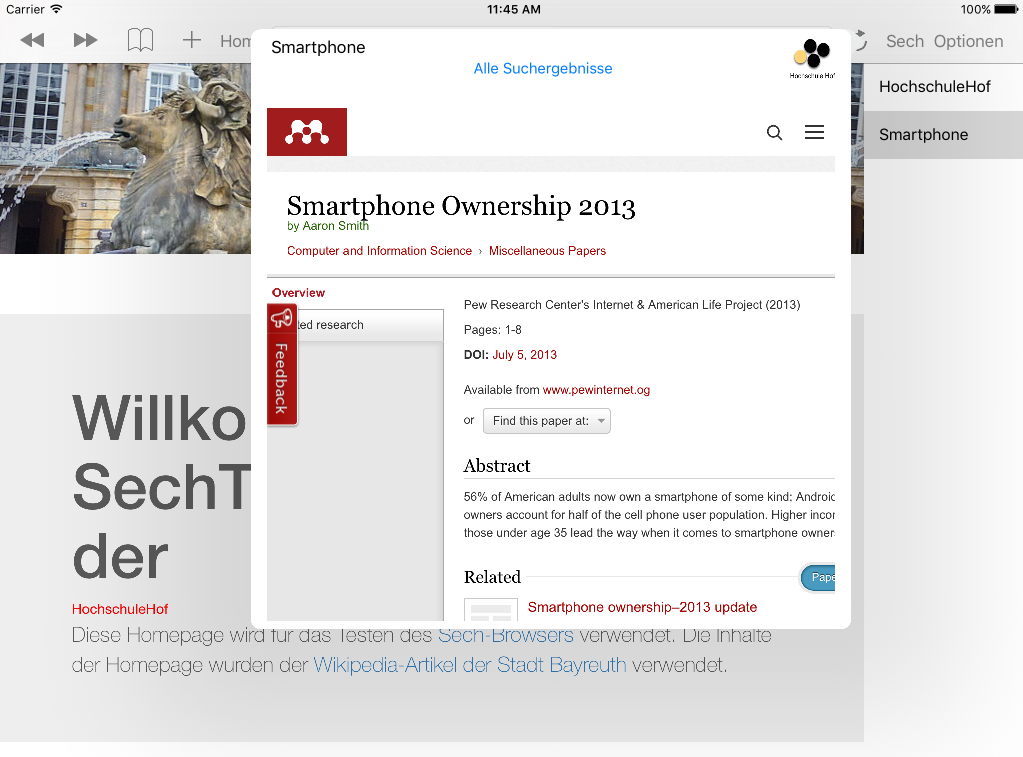
\includegraphics[height=0.4\textheight]{PopOver}
    \caption{Screenshot bei angeklicktem Search-Tag}
\end{figure}
In dem PopOverView wird oben links der Titel des angeklickten Search-Tags dargestellt. Daneben wird ein Button dargestellt, der eine weiter TableView enthält. Rechts oben wird noch das Logo des aktuellen Browsers angezeigt. Durch einen klick auf den Button \glqq Alle Suchergebnisse\grqq  wird eine neue TableView geöffnet, die weitere Suchergebnisse zu dem aktullen Suchbegriff enthält (vgl. Bild 2). Zum Öffnen der Tabelle wurde folgende Funktion auf den Button gelegt
\begin{lstlisting}
@IBAction func openTable(sender: AnyObject) {
        if let popover = popoverContent.popoverPresentationController {
            let viewForSource = sender as! UIView
            popover.sourceView = viewForSource
            popover.sourceRect = viewForSource.bounds
            popoverContent.preferredContentSize = CGSizeMake(400,500)
        }        
        self.presentViewController(popoverContent, animated: true,
         completion: nil)
    }
\end{lstlisting}
\begin{figure}[htb]
    \centering
    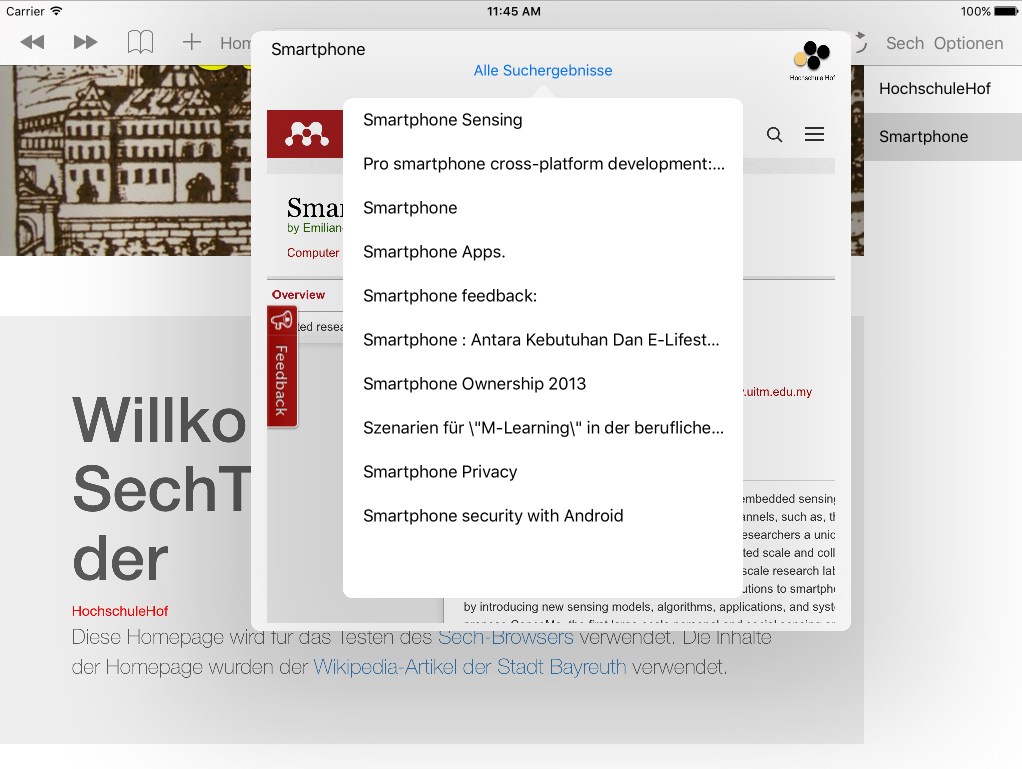
\includegraphics[height=0.4\textheight]{Table_in_PopOver}
    \caption{Screenshot bei angeklicktem Search-Tag}
\end{figure}
Durch diese Funktion, hat der Benutzer die Möglichkeit sich unterschiedliche Ergebnisse zu einem Search-Tag innerhalb eines Fensters anzeigen zu lassen. Durch einen Tap auf ein anderes Ergebnis in der Tabelle, läd der darunter liegende Webview neu. Um das Popover Fenster wieder zu schließen, muss der Benutzer nur innerhalb des Views tippen. Dadurch wird wieder der normale WebView angezeigt.
